\subsection{Code}

\subsubsection{Quick Start}
what is rotctl?
how to start it

\subsubsection{Raspberry Pi Setup}
how to configure the raspberry pi and connect to it


\subsubsection{code structure}
Main features:
- Rotctl
- Multithreading
- Sensors: magnetic encoder, quadrature
encoder, switches
- Separate driver modules: h-bridge, i2c
multiplexer etc.
- Position monitoring

how is it threadsafe?
how does it work?
where to configure the location?



\begin{figure}[h]
	\centering
	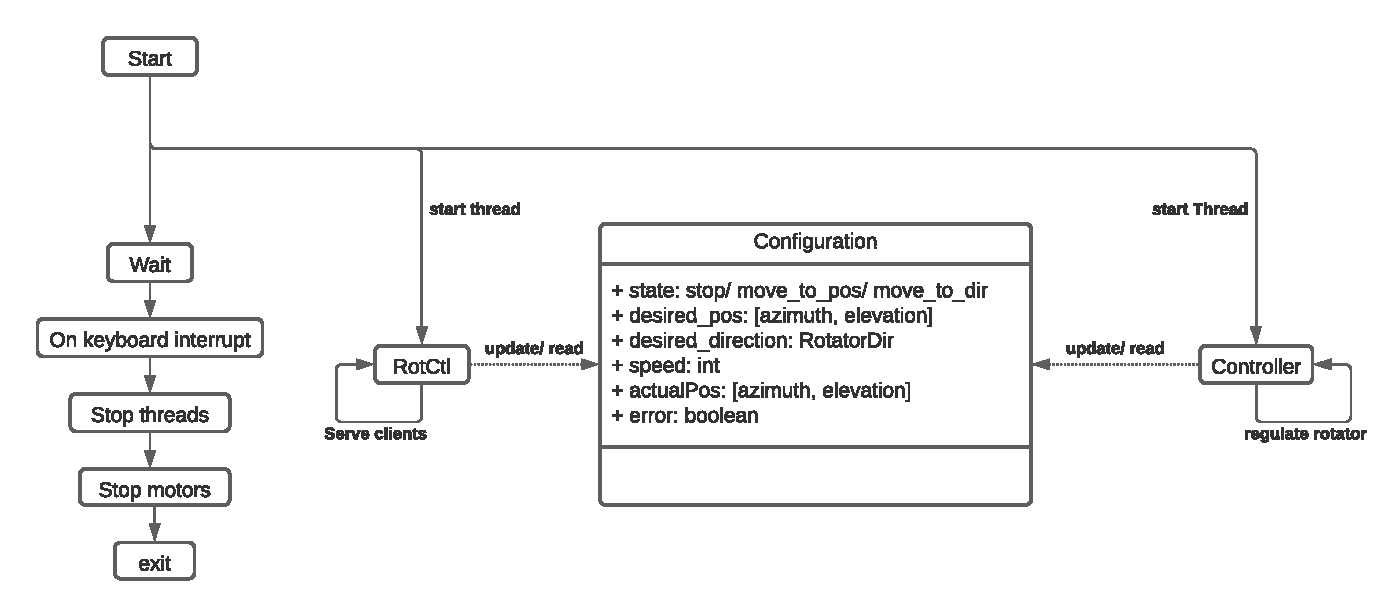
\includegraphics[width=\linewidth]{../art/Code flow chart.pdf}
	\caption{Raspberry pi HAT blockdiagramm}
\end{figure}



\begin{figure}[h]
	\centering
	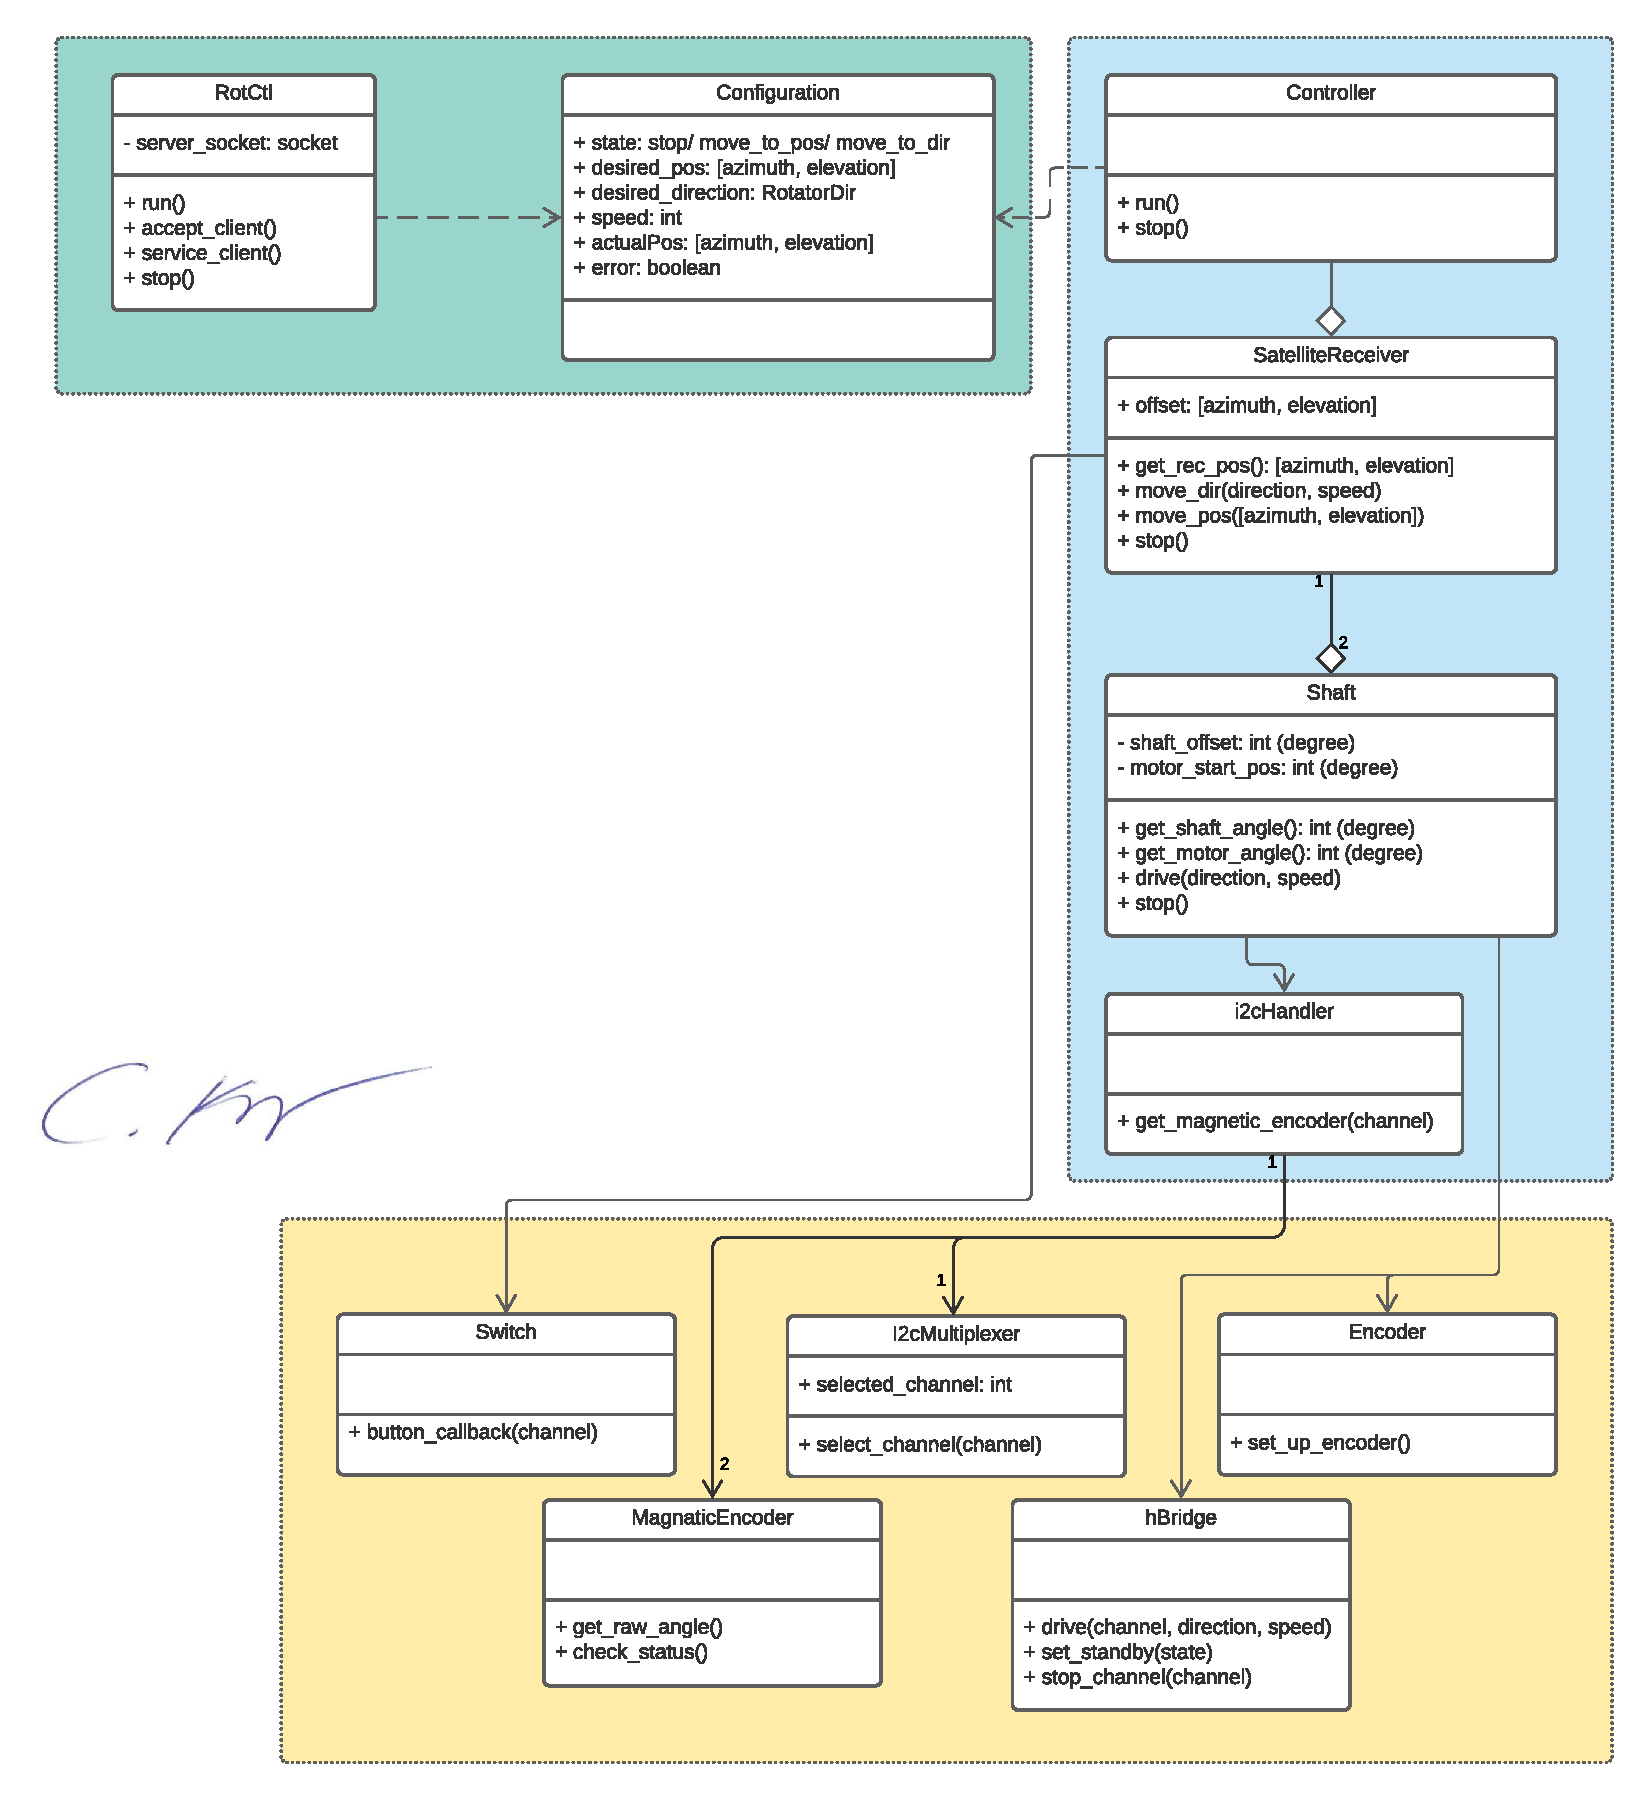
\includegraphics[scale=0.5]{../art/SatelliteReceiver.pdf}
	\caption{Code structure}
\end{figure}


\subsubsection{possible weak points}
- untested stuff
- 